\documentclass[12pt]{article}

% Packages
\usepackage[utf8]{inputenc} % Allows input of UTF-8 characters
\usepackage[T1]{fontenc} % Output font encoding for international characters
\usepackage{geometry} % For setting margins
\usepackage{times} % Times New Roman font
\usepackage{graphicx} % For including images
\usepackage{amsmath} % Math environments and symbols
\usepackage{hyperref}
\usepackage{float}

\newcommand{\vct}[1]{\mathbf{#1}}

\geometry{margin=1in}
\setlength{\parskip}{0.5em}

\title{
    Audio Wave Radiation with 3D Rigid Body Excitations\\
    \large Progress Report
}

\author{Karl Hiner\\khiner6@gatech.edu}
\date{\today}

\begin{document}

\maketitle

\section{Research topic and question}

I am investigating physical audio modeling of rigid bodies, in the field of dynamics.
Specifically, I will explore methods of estimating the time-varying sound pressure level at a point in a 3D environment with passive rigid bodies vibrating (and radiating audio waves) in a homogeneous medium (air) in response to excitations on their surface.

I am particularly interested in performance/accuracy tradeoffs, and aim to maximize (perceived) physical accuracy under the computational constraint of real-time audio generation on consumer hardware.

In a computationally constrained real-time interactive setting, what assumptions, models, and restrictions achieve results similar (in terms of quantitative and/or perceptual accuracy) to highly physically accurate (and computationally expensive) methods such as Finite-Difference Time-Domain (FDTD) estimation of acoustic wave propagation?

\section{Current setup}

I am adopting the physical setting described by Clarke et al. in \textit{RealImpact} \cite{clarke_realimpact_2023}, who created a dataset of 150,000 impact sound recordings of everyday objects with metadata including impact locations, microphone locations, contact forces, and material labels.

They constructed an acoustically treated recording environment with a gantry for moving microphones to precise positions in space, recording the sound of objects being struck by a hammer at various locations.

For each struck vertex, they move the gantry to 40 positions by rotating across 10 angles and 4 distances per angle.
Relative to the center of the mesh, the longest recorded distance is 1.23m, so this is the longest distance I consider in this project.

To allow near-free object vibrations and avoiding acoustic interference with the surface, they place objects on a mesh of polyester threads centered at the axis of rotation of the gantry and centered vertically along the gantry column holding 15 microphones.

The main component of my project is an interactive 3D simulation of this setup, in which a user can select an object mesh and a microphone position, and excite the object with a force at a vertex.
The application will support modeling arbitrary meshes (as long as they are valid volumetric surfaces), and excitation of any vertex.
Additionally, for the objects recorded by Clarke et al., the user may also measure and compare the simulated audio response to the recorded audio response at a selected microphone position and impact vertex.

\textbf{Methodology:} First, I transform a surface mesh into tetrahedral volumetric mesh.
I use the Finite Element Method (FEM) to estimate the mass, stiffness, and damping matrices of the rigid body from the tetrahedral mesh and material properties.
Then, I use an eigenvalue solver to find a preset number of most resonant vibrational modes, and generate audio using a parallel biquad filter bank tuned to resonate at the frequencies of each these modes.

To estimate the sound pressure level at the listener point due to acoustic waves radiating away from the object's surface, I plan to use the Boundary Element Method (BEM) as a somewhat more computationally efficient alternative to FDTD.
In either case (BEM or FDTD), acoustic radiation modeling will likely not be real-time viable without significant engineering effort.
In my proposal, I explored some potential methods and past works to inform efficient and accurate modeling of acoustic radiation in the context of rigid body vibrations of a single, stationary object.
However, exactly which method(s) I will apply, if any, in the context of the interactive simulation application is still an open question.

\section{Code repository}

The code for this project can be found at \href{https://github.com/khiner/MeshEditor}{https://github.com/khiner/MeshEditor}.

\section{Current status}

Currently, the application supports loading and rendering 3D meshes, selecting a microphone position, and triggering the \textit{RealImpact} recording of the mesh struck at a selected vertex.
I have also ported all necessary FEM and modal audio generation code I implemented for a \href{https://github.com/GATech-CSE-6730-Spring-2023-Project/mesh2audio}{project in a previous class}.

The major components remaining are:
\begin{itemize}
    \item Finishing the modal audio interface and implementing methods and user interface for comparing simulated audio with recorded audio (including waveform and spectrogram displays).
    \item Incorporating damping estimations into the FEM model. (Currently, the scale of resonator damping is the same for all objects, and this can have an important effect on the audio response.)
    \item Implementing an acoustic radiation estimation model.
\end{itemize}

\section{Difficulties and change of plans}

My biggest challenge is in deciding how to balance my goals of an interactive application, and the target deliverables of the poster presentation.
I am motivated (outside the context of this course!) to implement this simulation application, but I want to avoid re-implementing many ascpects e.g. in Python to generate standard static plots, etc.
I am considering bringing my laptop and a pair of headphones to the poster session to demonstrate the interactive application, and I'm looking for feedback on this concern (which I will bring up in office hours).

\section{List of figures}

The primary figures I plan to present are of comparisons between spectra of simulated and recorded audio waveforms, with an emphasis on comparing the salient resonant modes.

Here are some images of application currently:

Below, on the left \ref{fig:mic_overhead} is an overhead view of the "microphone" listener positions surrounding a sound object, and on the right \ref{fig:mic_overhead_compare} is an image from \textit{RealImpact} \cite{clarke_realimpact_2023} for comparison.
The following image is of a skillet mesh selected for user interaction and surrounded by microphones \ref{fig:skillet}.

\begin{figure}[H]
    \centering
    \begin{minipage}[t]{0.45\linewidth}
        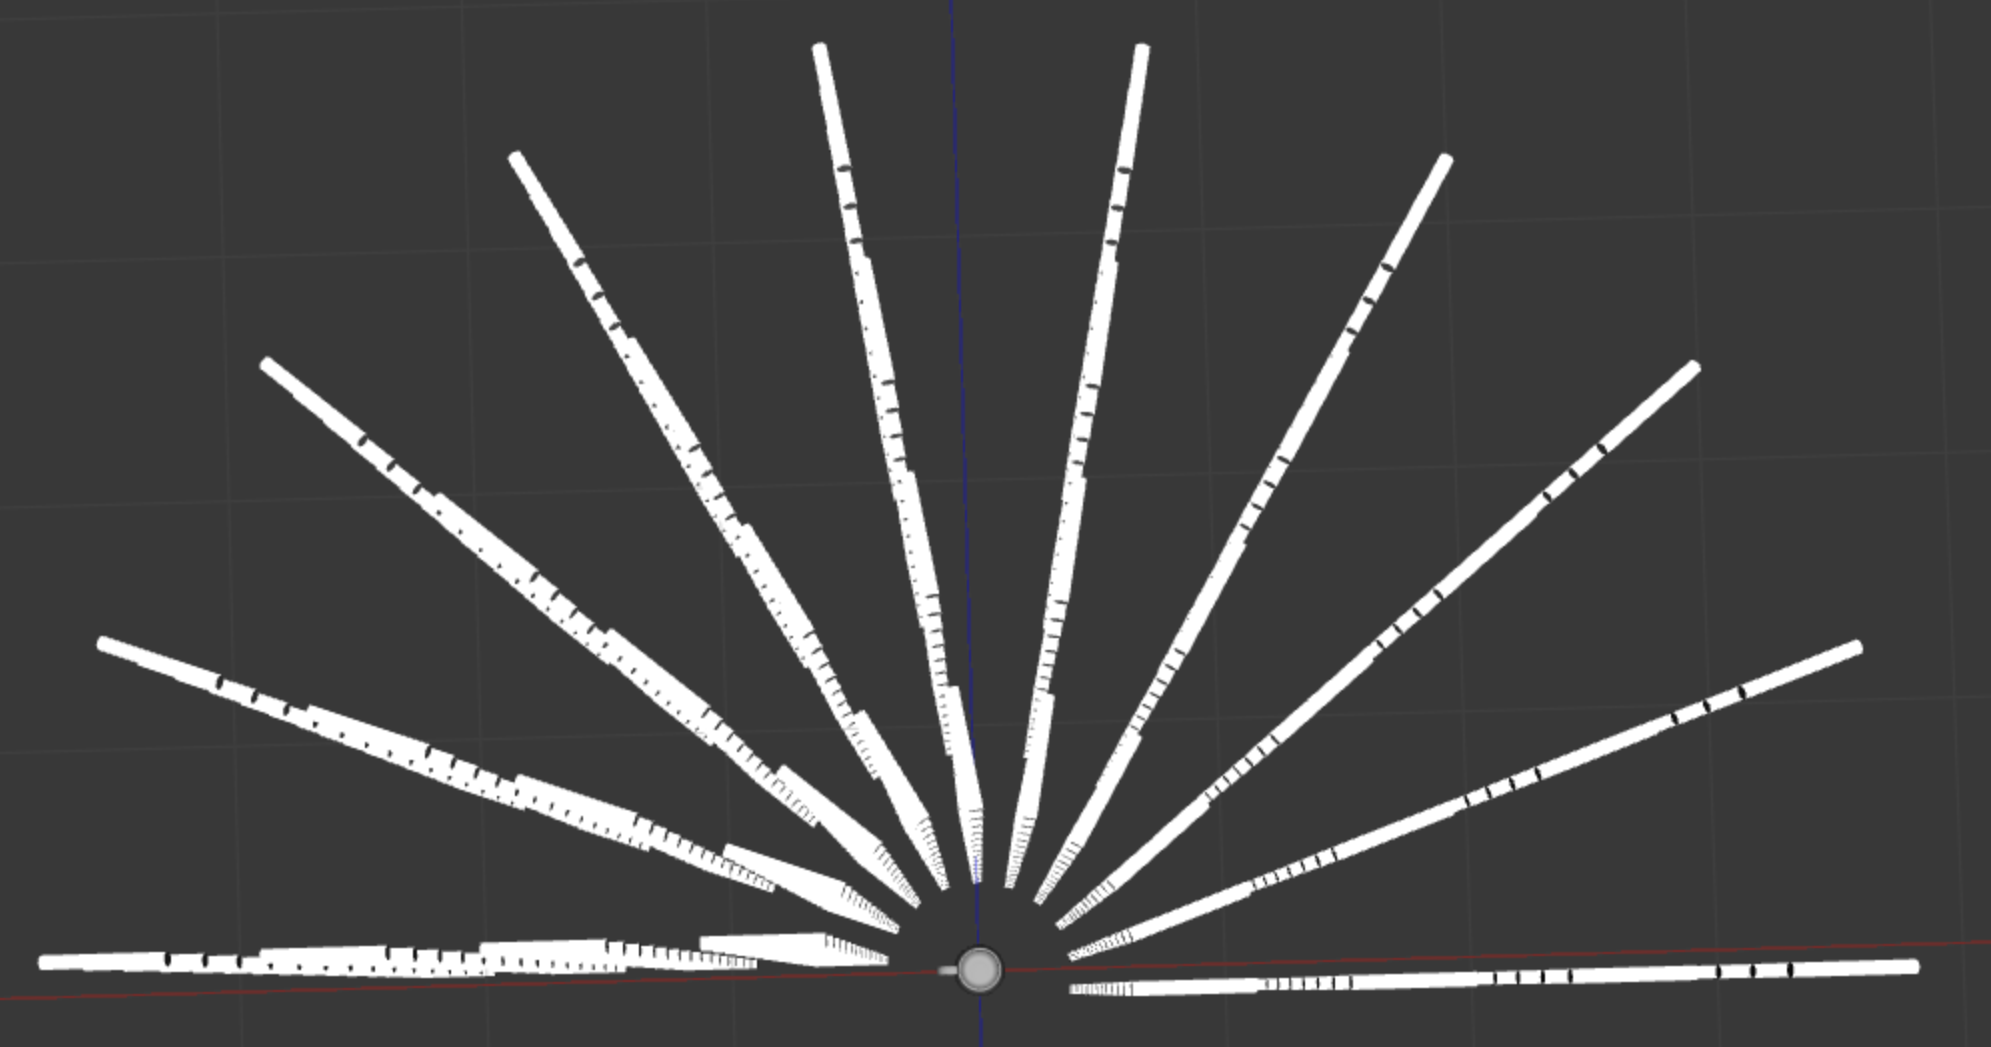
\includegraphics[width=\linewidth]{overhead_mic_view.png}
        \caption{Overhead view of microphone listener positions and cup mesh}
        \label{fig:mic_overhead}
    \end{minipage}
    % \hfill
    \begin{minipage}[t]{0.45\linewidth}
        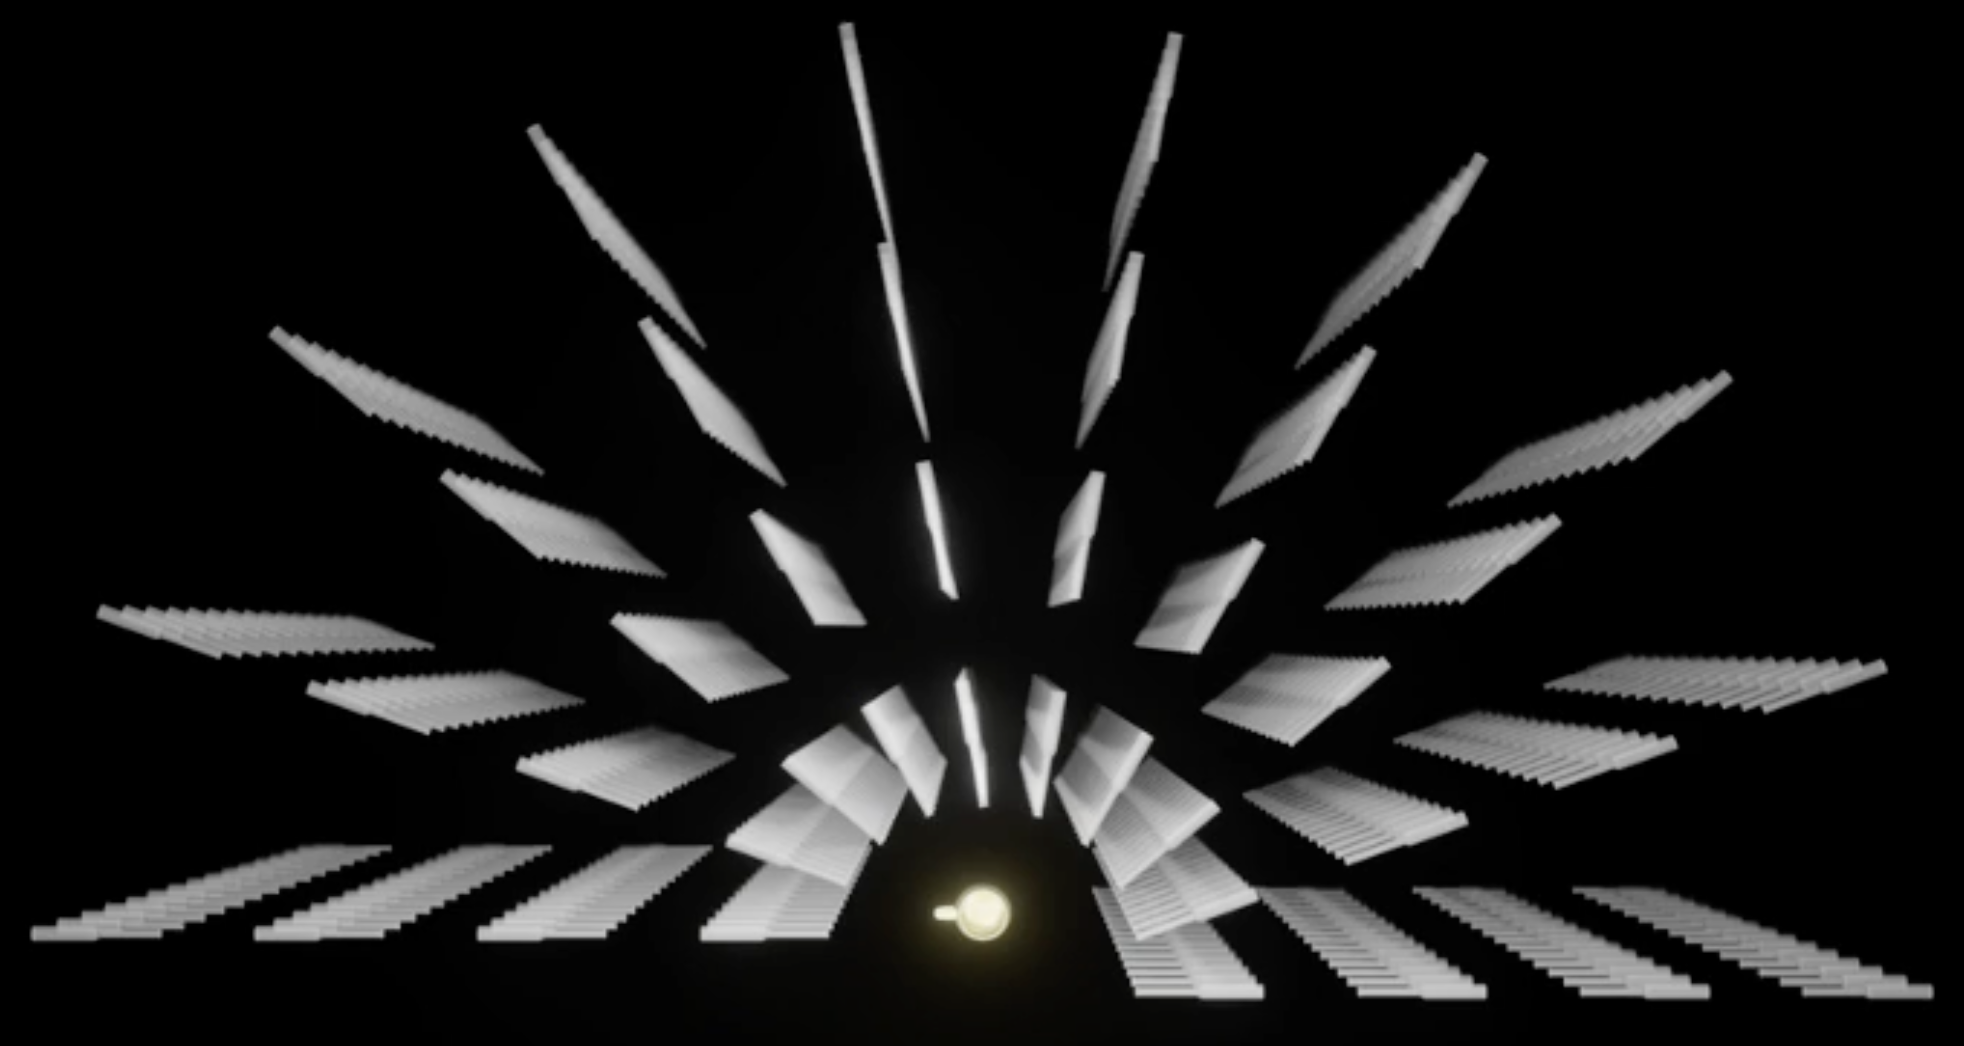
\includegraphics[width=\linewidth]{overhead_mic_comparison.png}
        \caption{Image from RealImpact}
        \label{fig:mic_overhead_compare}
    \end{minipage}
\end{figure}


\begin{figure}[H]
    \centering
    \begin{minipage}[t]{0.65\linewidth}
        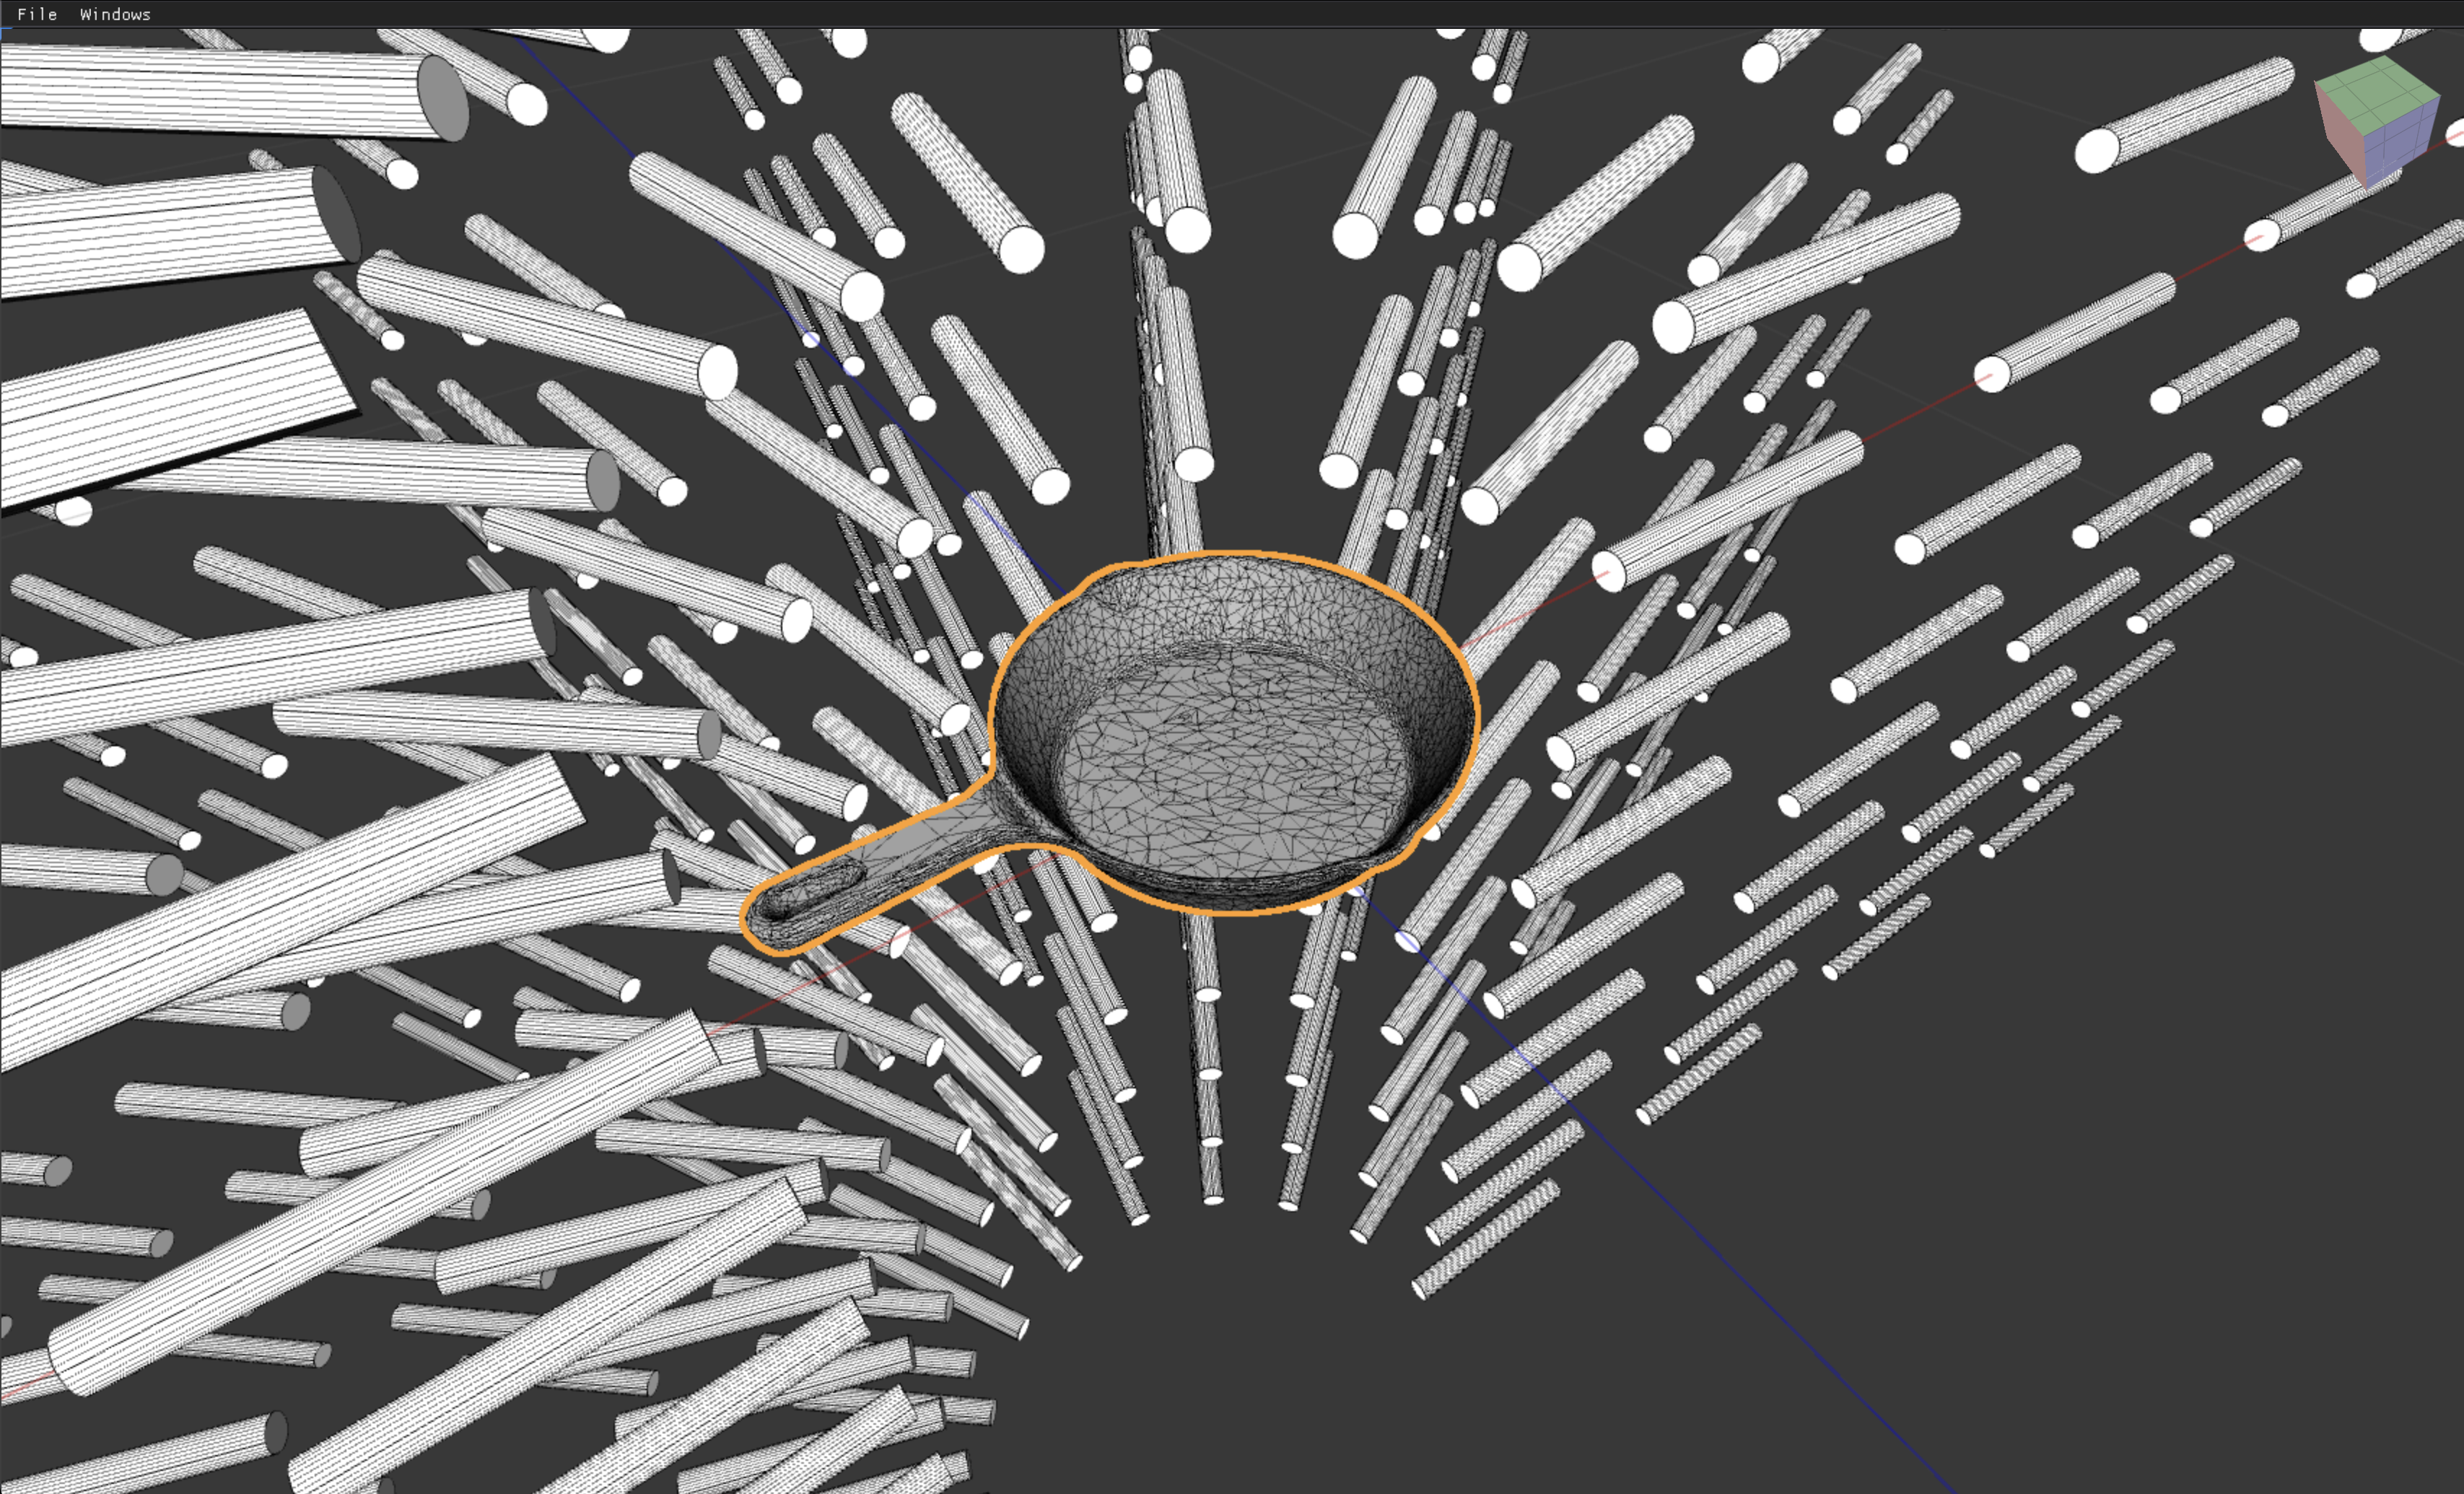
\includegraphics[width=\linewidth]{real_impact_skillet.png}
        \caption{Selected skillet mesh surrounded by microphones}
        \label{fig:skillet}
    \end{minipage}
\end{figure}

\section{Background on Modal Vibration Models}

We briefly summarize the necessary background on modal vibration analysis here, and refer the reader to a suitable text \cite{shabana1990theory}. The linear elastodynamic equation for a finite element model \cite{zienkiewicz1977finite},

\begin{equation}
    M\ddot{u} + C\dot{u} + Ku = F, \tag{1}
\end{equation}

describes the displacements $u=u(t)$ of $N$ nodes within a volume. The displacement field $u$ is expanded in a modal displacement basis

\begin{equation}
    u(t) = \Phi q(t), \tag{2}
\end{equation}

where $\Phi$ denotes the model's modal matrix, a matrix whose $i$th column $\Phi_i$ represents the $i$th mode shape, and $q = q(t)$ are the corresponding modal amplitudes, i.e., $q_i$ is the modal amplitude of mode shape $\Phi_i$. An important property is that the modal matrix $\Phi$ is independent of time, and completely characterized by values at mesh vertices.

Substituting (2) into (1) and premultiplying by $\Phi^T$ yields

\begin{equation}
    M_q \ddot{q} + C_q \dot{q} + K_q q = Q, \tag{3}
\end{equation}

in which

\begin{equation}
    M_q = \Phi^T M \Phi = \operatorname{diag}(m_i), \tag{4}
\end{equation}

\begin{equation}
    K_q = \Phi^T K \Phi = \operatorname{diag}(k_i), \tag{5}
\end{equation}

\begin{equation}
    C_q = \Phi^T C \Phi, \tag{6}
\end{equation}

\begin{equation}
    Q = \Phi^T F. \tag{7}
\end{equation}

where all of $M_q$ and $K_q$ are diagonal matrices, but for general damping $C_q$ is dense. If we make the common assumption of proportional (Rayleigh) damping

\begin{equation}
    C = \alpha M + \beta K \Rightarrow C_q = \operatorname{diag}(\alpha m_i + \beta k_i),
\end{equation}

then the system of ODEs are completely decoupled by the modal transformation. This allows the motions due to individual modes to be computed independently and combined by linear superposition.

The system of decoupled ordinary differential equations may be written as

\begin{equation}
    \ddot{q}_i + 2\xi_i \omega_i \dot{q}_i + \omega_i^2 q_i = \frac{Q_i}{m_i}, \quad i = 1..n, \tag{8}
\end{equation}

where the undamped natural frequency of vibration is

\begin{equation}
    \omega_i = \sqrt{\frac{k_i}{m_i}} \quad \text{(in radians)}, \tag{9}
\end{equation}

and the dimensionless modal damping factor is

\begin{equation}
    \xi_i = \frac{c_i}{2m_i\omega_i} = \frac{1}{2} \left(\frac{\alpha}{\omega_i} + \beta\omega_i\right). \tag{10}
\end{equation}

We are interested in underdamped systems for which visible damped vibration occurs, and this corresponds to $\xi_i \in (0, 1)$.

Finally, for a system starting from rest at $t=0$, the solution for the $i$th mode due to forcing $Q_i(t)$ is

\begin{equation}
    q_i(t) = \int_{0}^{t} e^{-\xi_i \omega_i (t-\tau)} \sin \omega_{di} (t- \tau) \frac{Q_i(\tau)}{m_i \omega_{di}} \, d\tau, \tag{11}
\end{equation}

where the observed damped natural frequency is

\begin{equation}
    \omega_{di} = \omega_i \sqrt{1 - \xi_i^2}. \tag{12}
\end{equation}


\bibliographystyle{plain}
\bibliography{bibliography}

\end{document}
